%
% 第五章
%
\chapter{硬盘文件安全加载方案测试及分析}
\label{cha:test}
有了三四章节的理论和代码基础,本章将在此基础上,逐步进行实验验证分析。验证内容包括,DXE阶段驱动程序度量功能
的验证、BDS阶段硬盘文件度量功能的验证、UEFI系统中BMC驱动程序的连通性验证、通过EDKII编译生成的fd固件文件格式
的验证以及DXE阶段修改驱动程序加载顺序的验证。下面将先对实验环境进行介绍,以及选用的原因。

%
% 5.1节
%
\section{实验环境}

\subsection{申威6A服务器真机环境}
实验的真机环境是可信固件实验室提供的申威6A型服务器,实验环境包括了固件的编译环境以及服务器中BMC提供的fd固件
文件烧写环境,具体信息如下:
\par (1)固件编译系统环境:Ubuntu 10.04版本,并配置uuid-dev-2.17包
\par (2)固件编译工具:原版gcc4.4.3,和申威定制的swgcc-4.5.3-交叉编译器
\par (3)EDKII信息:带有申威定制包SenweiPkg的EDKIIR13995版本
\par (4)BMC烧写环境:Ubuntu 16.04版本和Firefox浏览器
\par Ubuntu 10.04版本的选择主要原因在于它提供的C语言库函数版本问题,由于swgcc-4.5.3-交叉编译器的特殊性,
需要特定库版本的支持,在以往实验中这一点经过验证。由于真机环境上运行的固件是经过申威ALPHA64架构处理器指令集定
制的,因此根据编译环境的特殊性做一些编译方法的介绍。交叉编译器的设置是通过linux系统软链接的方式实现的:

\begin{lstlisting}
ln -s sw_64sw2-unknown-linux-gnu-ar swar
ln -s sw_64sw2-unknown-linux-gnu-as swas
ln -s sw_64sw2-unknown-linux-gnu-gcc swgcc
ln -s sw_64sw2-unknown-linux-gnu-ld swld
ln -s sw_64sw2-unknown-linux-gnu-objcopy swobjcopy    
\end{lstlisting}

通过以上命令分别将申威定制版本的gcc编译器链接到官方版本gcc的调用名称上面,来实现编译命令的调用。

\begin{figure}[htb]
    \label{ffs_format}
    % 调整图片与上文的垂直距离 %
    \vspace{0cm}   
    % 调整图片图片与中文标题、中文标题与英文标题距离 %
    \setlength{\abovecaptionskip}{0.3cm}
    % 引用/fig/目录中的图片文件 %
	\centering
    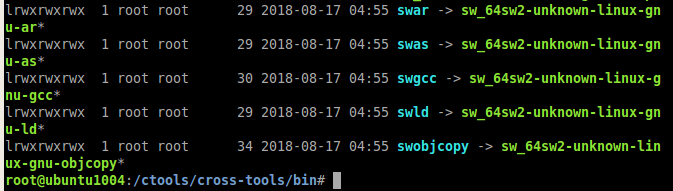
\includegraphics[width=12cm]{cross_tools.png}
    % 中文标题 %
    \caption*{图 5-1 编译器软连接}
    % 调整图片英文标题与下文距离(本文标准为-0.7cm) %
    \setlength{\belowcaptionskip}{-0.7cm}
    % 英文标题 %
    \caption*{Figure 5-1 Compiler Soft Link}
\end{figure}

图5-1所示的是查看软链接的修改效果。接下来是交叉编译申威固件程序的过程,首先需要使用原版gcc4.4.3编译器进行
edksetup程序的初始化工作,这个程序的目的在于为正在打开着的终端窗口设置好通过build编译时一切所需的环境变量
及一些通过C语言根据UEFI规范自动生成的代码内容。

\begin{figure}[htb]
    \label{ffs_format}
    % 调整图片与上文的垂直距离 %
    \vspace{0cm}   
    % 调整图片图片与中文标题、中文标题与英文标题距离 %
    \setlength{\abovecaptionskip}{0.3cm}
    % 引用/fig/目录中的图片文件 %
	\centering
    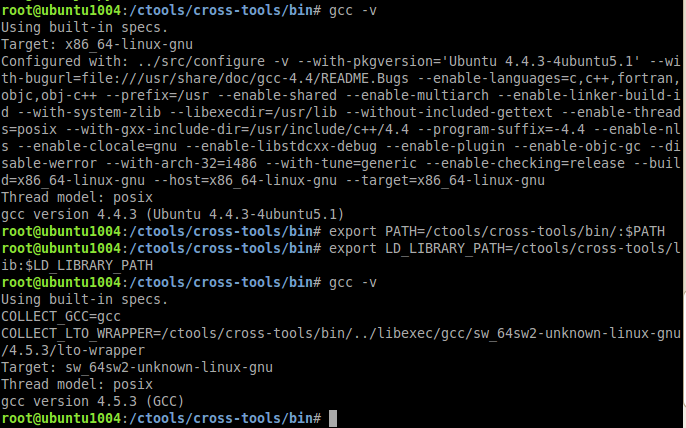
\includegraphics[width=12cm]{swgcc.png}
    % 中文标题 %
    \caption*{图 5-2 GCC版本切换过程}
    % 调整图片英文标题与下文距离(本文标准为-0.7cm) %
    \setlength{\belowcaptionskip}{-0.7cm}
    % 英文标题 %
    \caption*{Figure 5-2 GCC version switching process}
\end{figure}

如图5-2所示,是通过export改变环境变量的命令,将我们设置好的swgcc交叉编译器软链接目录添加到两个系统环境
变量中的过程,通过这样的方式,就可以实现用gcc 4.4.3版本进行edksetup程序的运行,并用swgcc交叉编译器进行
平台dsc文件的构建编译过程。具体编译过程,采用linux SHELL脚本的方式进行使用,如图5-3。

\begin{figure}[H]
    \label{ffs_format}
    % 调整图片与上文的垂直距离 %
    \vspace{0cm}   
    % 调整图片图片与中文标题、中文标题与英文标题距离 %
    \setlength{\abovecaptionskip}{0.3cm}
    % 引用/fig/目录中的图片文件 %
	\centering
    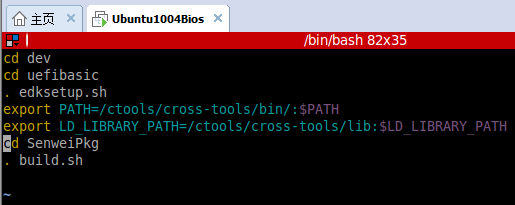
\includegraphics[width=12cm]{sw_sh_file.png}
    % 中文标题 %
    \caption*{图 5-3 交叉编译功能的终端程序}
    % 调整图片英文标题与下文距离(本文标准为-0.7cm) %
    \setlength{\belowcaptionskip}{-0.7cm}
    % 英文标题 %
    \caption*{Figure 5-3 Cross compile shell program}
\end{figure}

\begin{figure}[htb]
    \label{ffs_format}
    % 调整图片与上文的垂直距离 %
    \vspace{0cm}   
    % 调整图片图片与中文标题、中文标题与英文标题距离 %
    \setlength{\abovecaptionskip}{0.3cm}
    % 引用/fig/目录中的图片文件 %
	\centering
    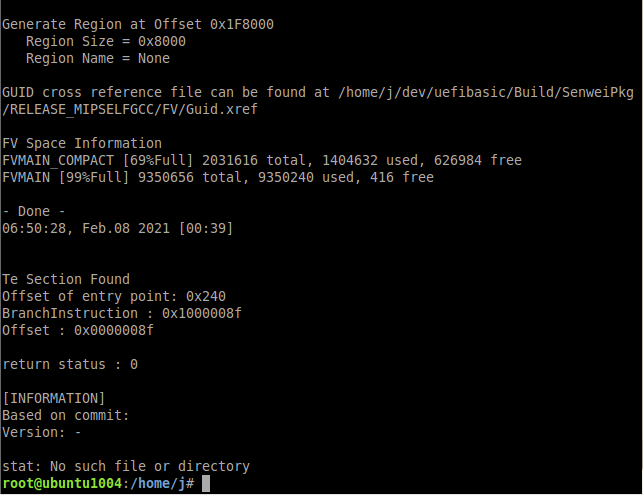
\includegraphics[width=12cm]{compile_res.png}
    % 中文标题 %
    \caption*{图 5-4 交叉编译结果}
    % 调整图片英文标题与下文距离(本文标准为-0.7cm) %
    \setlength{\belowcaptionskip}{-0.7cm}
    % 英文标题 %
    \caption*{Figure 5-4 Cross compile result}
\end{figure}

其中图5-3为开发的脚本语言编译程序,图5-4为最终的固件编译结果。

\subsection{UEFI Windwos模拟环境}
与真机环境对应的是Windows系统下的UEFI模拟运行环境,建立这个环境的目的在于,能够简化固件开发过程中调试的
复杂程度,通过模拟环境测试一些硬件结构不相关的功能模块运行效果,增加开发效率。其中具体信息如下:
\par (1)固件编译系统环境:Windows 10
\par (2)固件编译工具:VS2008
\par (3)EDKII信息:EDKIIR13995版本
\par 模拟环境的编译较为简单因此不做详细说明,编译效果图如图5-5。其中是GenFds命令生成最终fd固件文件的过程,
固件名称为NT32.fd。

\begin{figure}[htb]
    \label{ffs_format}
    % 调整图片与上文的垂直距离 %
    \vspace{0cm}   
    % 调整图片图片与中文标题、中文标题与英文标题距离 %
    \setlength{\abovecaptionskip}{0.3cm}
    % 引用/fig/目录中的图片文件 %
	\centering
    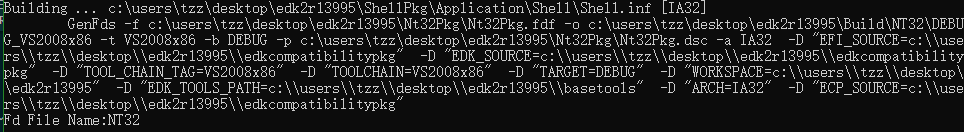
\includegraphics[width=12cm]{win_compile.png}
    % 中文标题 %
    \caption*{图 5-5 UEFI模拟环境编译结果}
    % 调整图片英文标题与下文距离(本文标准为-0.7cm) %
    \setlength{\belowcaptionskip}{-0.7cm}
    % 英文标题 %
    \caption*{Figure 5-5 UEFI simulation environment compilation results}
\end{figure}

%
% 5.2节
%
\section{驱动度量功能验证}
本文中在DXE阶段加载的可信度量驱动程序,主要用来度量四个UEFI文件系统协议栈驱动程序,并向BMC发送度量日志。
基于以上功能对可信度量驱动程序进行测试。

\subsection{测试目的}
该可信度量功能对DXE阶段特定驱动的度量方法存在普遍性,给出了根据现有UEFI驱动加载的设计理念,自定义度量驱动
内容的方法。该过程的正确性直接影响了BDS阶段加载硬盘文件的安全可信性。

\subsection{测试步骤}
(1)首先编写具有上述五个模块的DXE阶段可信度量驱动程序,并将其模块INF文件通过引用的方式添加到将要编译的申威平台
描述文件dsc文件中。
\par (2)然后通过本章第一节中的方法,对申威UEFI组件进行交叉编译。
\par (3)通过BMC芯片提供的网卡端口服务程序,用单独的客户端主机访问服务器上的网卡端口,此过程设置客户端
静态IP,设置成与BMC提供的服务IP同一网段内,并烧写UEFI BIOS固件文件到服务器的闪存芯片中。
\par (4)服务器上电并按电源按钮,进入UEFI BIOS启动流程,过程中将根据DXE阶段依赖,加载并度量四个特定驱动
程序。
\par (5)通过与步骤(3)同样的方法,通过网卡用客户端访问BMC,此时客户端需要安装default-jdk环境,并安装了
Maintance维护工具。通过lazyrrk 30 0命令获取BMC日志信息,其中包括驱动的度量日志。

\subsection{测试过程}
首先将经过交叉编译生成的SENWEI.fd文件通过BMC功能烧写如BIOS闪存中,如图5-6所示。将通过通过2400的控制器访问
并烧写提供的BIOS固件文件,烧写过程需要开机烧写,否则烧写失败。

\begin{figure}[H]
    \label{ffs_format}
    % 调整图片与上文的垂直距离 %
    \vspace{0cm}   
    % 调整图片图片与中文标题、中文标题与英文标题距离 %
    \setlength{\abovecaptionskip}{0.3cm}
    % 引用/fig/目录中的图片文件 %
	\centering
    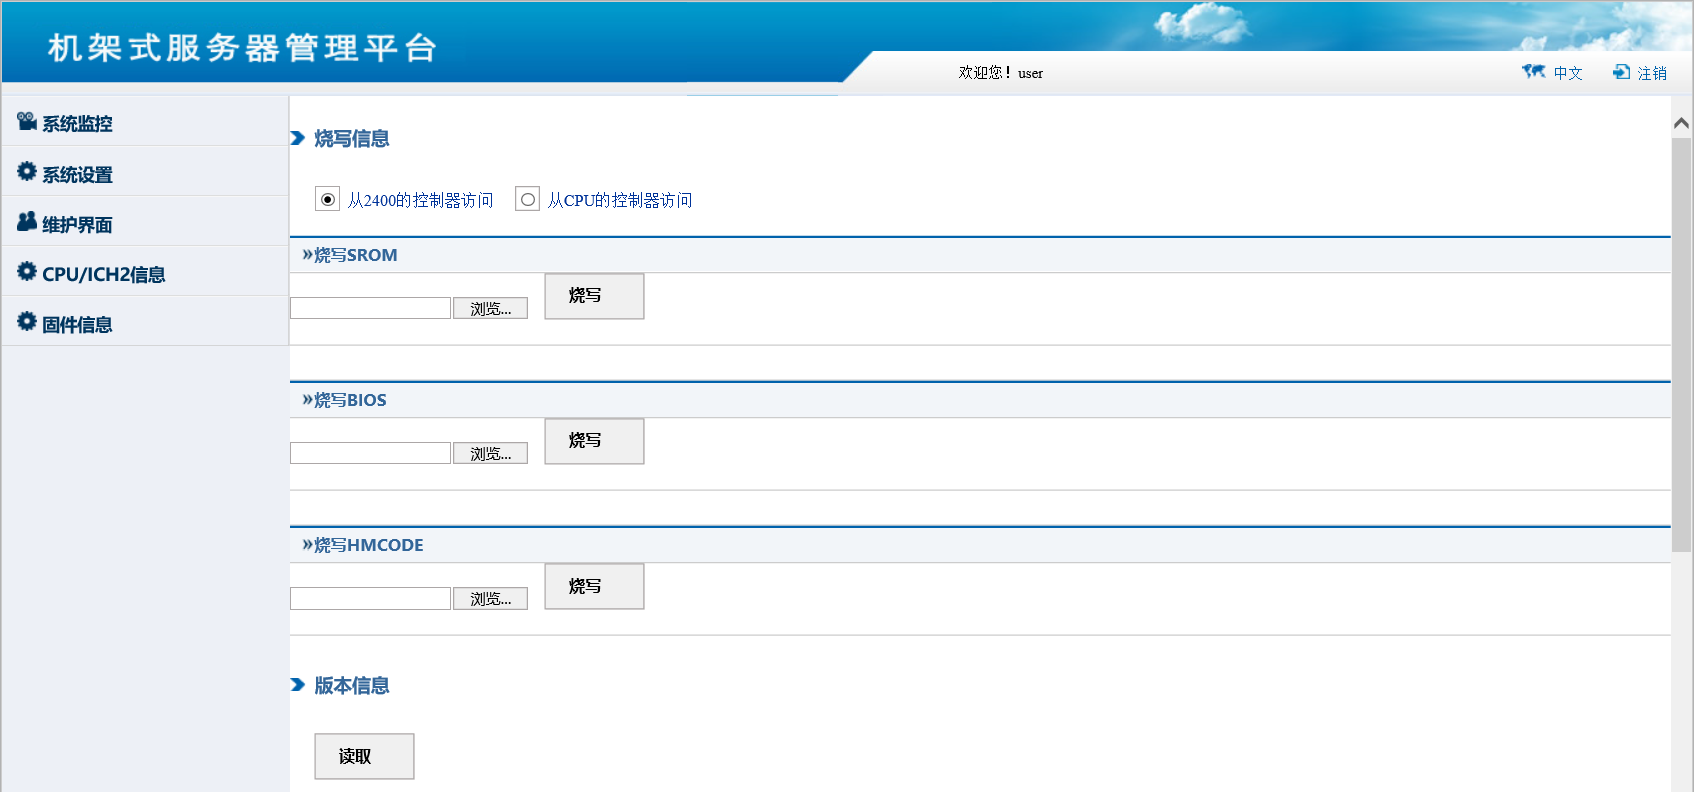
\includegraphics[width=12cm]{bmc.png}
    % 中文标题 %
    \caption*{图 5-6 BMC烧写固件界面}
    % 调整图片英文标题与下文距离(本文标准为-0.7cm) %
    \setlength{\belowcaptionskip}{-0.7cm}
    % 英文标题 %
    \caption*{Figure 5-6 BMC firmware interface}
\end{figure}

然后就是驱动度量日志的查看过程,通过安装的维护工具访问BMC特定端口,并通过linux系统中的重定向输出功能将读取
到的日志信息,写入指定的文件中。图5-7所示为四个特定驱动的度量日志。

\begin{figure}[H]
    \label{ffs_format}
    % 调整图片与上文的垂直距离 %
    \vspace{0cm}   
    % 调整图片图片与中文标题、中文标题与英文标题距离 %
    \setlength{\abovecaptionskip}{0.3cm}
    % 引用/fig/目录中的图片文件 %
	\centering
    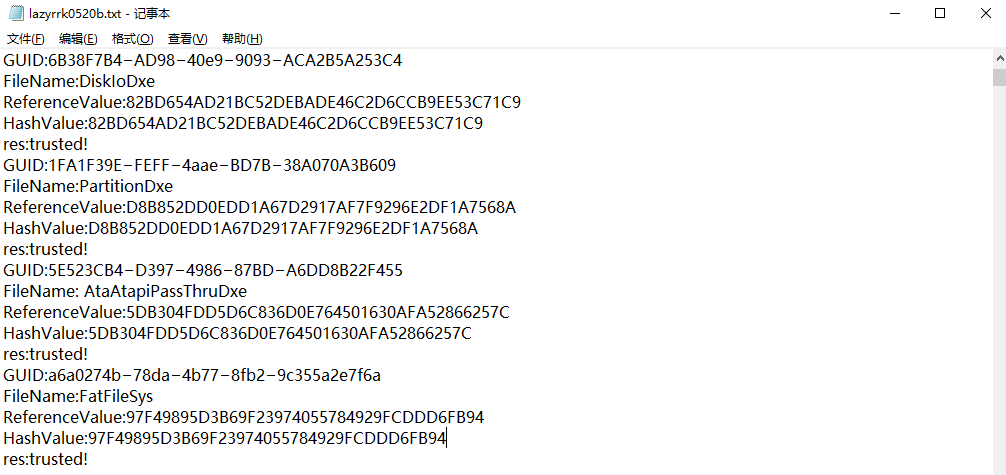
\includegraphics[width=12cm]{log.png}
    % 中文标题 %
    \caption*{图 5-6 驱动度量日志}
    % 调整图片英文标题与下文距离(本文标准为-0.7cm) %
    \setlength{\belowcaptionskip}{-0.7cm}
    % 英文标题 %
    \caption*{Figure 5-6 Driver mesurement log}
\end{figure}

%
% 5.3节
%
\section{BMC驱动连通性验证}

\subsection{测试目的}
在可信度量驱动程序的开发过程中,需要一个从BMC系统取出基准值的过程,通过单独测试UEFI BIOS中BMC驱动程序
的连通性有助于单独功能地调试可信度量驱动,保证BMC驱动的可用性。

\subsection{测试步骤}
(1)编写DXE阶段的BMC驱动程序,编写BMC的BIOS SHELL命令,可输入IPMI指令和内容,并获取到BMC返回的结果。
将BMC驱动的INF文件添加到申威平台描述文件dsc文件中。
\par (2)然后通过本章第一节中的方法,对申威UEFI组件进行交叉编译。
\par (3)通过BMC提供的烧写功能烧写BIOS固件。
\par (4)服务器上电并按下开机按钮,按F12进入到UEFI界面并通过SHELL启动方式进入到UEFI SHELL环境。
\par (5)输入开发好的BMC命令,并从SHELL界面查看结果。

\subsection{测试过程}
虽然SHELL作为UEFI BIOS系统中的一个上层用户程序,但作为BIOS来说,并不区分内核和用户的内存访问区域,因此
SHELL程序依然可以访问到UEFI初始化的一切系统资源,为驱动的测试提供了基础。如图5-7所示,是通过名为bmc\_kcs
的SHELL命令发送并接收数据的过程。

\begin{figure}[H]
    \label{ffs_format}
    % 调整图片与上文的垂直距离 %
    \vspace{0cm}   
    % 调整图片图片与中文标题、中文标题与英文标题距离 %
    \setlength{\abovecaptionskip}{0.3cm}
    % 引用/fig/目录中的图片文件 %
	\centering
    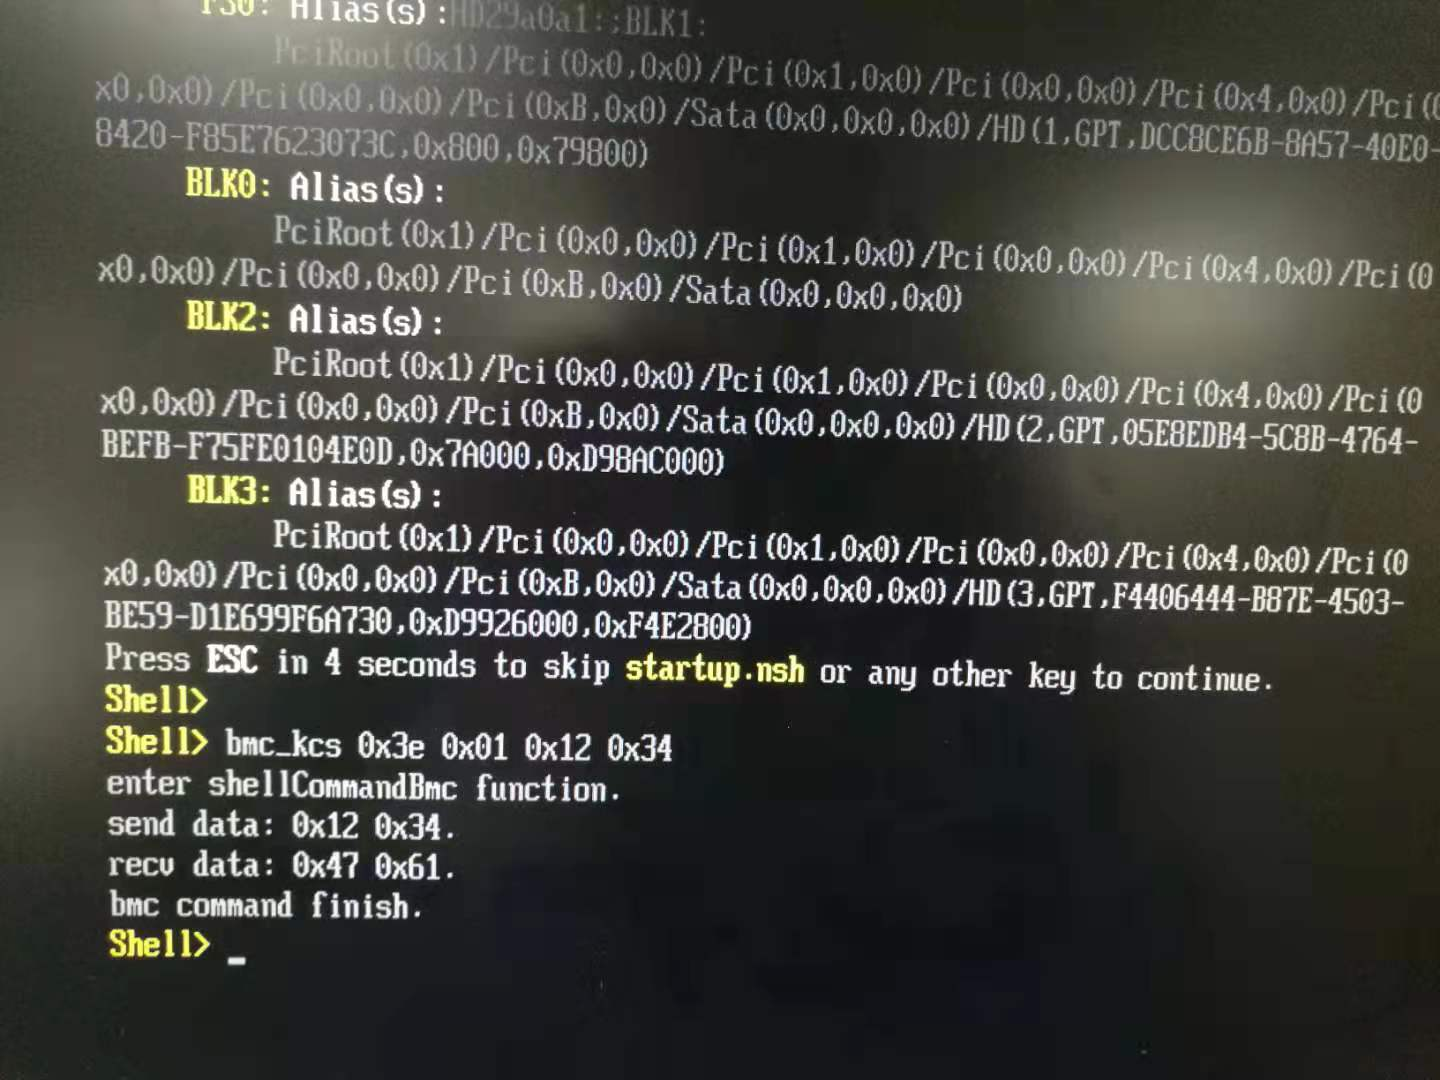
\includegraphics[width=12cm]{bmc_kcs.png}
    % 中文标题 %
    \caption*{图 5-7 BMC命令运行结果}
    % 调整图片英文标题与下文距离(本文标准为-0.7cm) %
    \setlength{\belowcaptionskip}{-0.7cm}
    % 英文标题 %
    \caption*{Figure 5-7 BMC command results}
\end{figure}

%
% 5.4节
%
\section{依赖表达式验证}

\subsection{测试目的}
依赖表达式是PEI和DXE驱动加载阶段的加载顺序的主要依据,他与优先级文件对应,属于弱类型。通过验证依赖表达式
在固件文件中的存储以及在驱动加载过程中如何控制加载顺序,可确保可信度量驱动在需被度量的特定驱动前加载,保证
度量功能的可用性。

\subsection{测试步骤}
(1)在DXE core代码的调度器程序中添加向SHELL输出的DEBUG函数。
\par (2)通过配置VS2008来对UEFI BIOS进行编译,得到NT32.fd文件。
\par (3)通过UEFITool这个fd文件解析程序,对NT32.fd进行解析。
\par (4)运行模拟程序的入口点exe可执行文件,根据SHELL输出的DEBUG信息得到依赖表达式解析过程。

\subsection{测试过程}
在经过VS2008编译器编译后生成Windows平台的UEFI模拟环境固件文件,通过UEFITool工具查看到的文件信息如下。

\begin{figure}[H]
    \label{ffs_format}
    % 调整图片与上文的垂直距离 %
    \vspace{0cm}   
    % 调整图片图片与中文标题、中文标题与英文标题距离 %
    \setlength{\abovecaptionskip}{0.3cm}
    % 引用/fig/目录中的图片文件 %
	\centering
    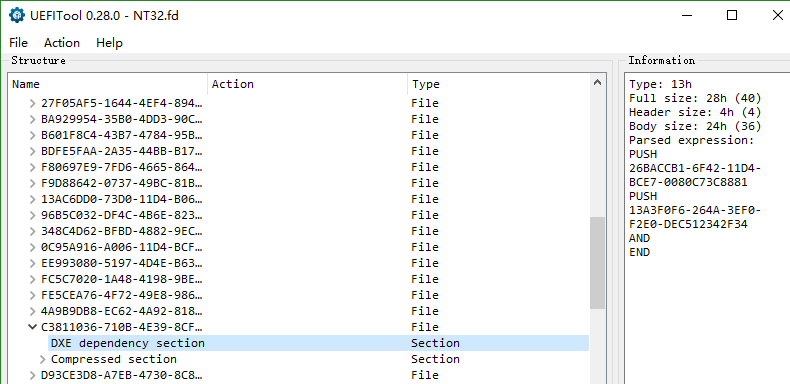
\includegraphics[width=12cm]{fd_depex.png}
    % 中文标题 %
    \caption*{图 5-8 固件文件依赖区域内容}
    % 调整图片英文标题与下文距离(本文标准为-0.7cm) %
    \setlength{\belowcaptionskip}{-0.7cm}
    % 英文标题 %
    \caption*{Figure 5-8 FD file dependency section content}
\end{figure}

图5-8所示的是DXE阶段的TimerDxe驱动在FV格式的固件卷中的dependency section中的内容,两个GUID分别代表两个
协议,他们对应的名称是gEfiCpuArchProtocolGuid和gEfiPcdProtocolGuid。下面是运行过程中TimerDxe驱动对应
的加载过程日志信息显示。

\begin{figure}[H]
    \label{ffs_format}
    % 调整图片与上文的垂直距离 %
    \vspace{0cm}   
    % 调整图片图片与中文标题、中文标题与英文标题距离 %
    \setlength{\abovecaptionskip}{0.3cm}
    % 引用/fig/目录中的图片文件 %
	\centering
    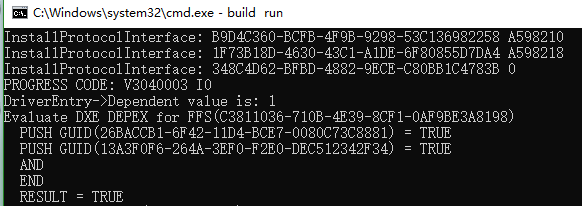
\includegraphics[width=12cm]{timer_depex.png}
    % 中文标题 %
    \caption*{图 5-9 驱动加载过程中的日志信息}
    % 调整图片英文标题与下文距离(本文标准为-0.7cm) %
    \setlength{\belowcaptionskip}{-0.7cm}
    % 英文标题 %
    \caption*{Figure 5-9 Log information during driver loading}
\end{figure}

图5-9显示的是在通过SecMain.exe入口点或命令build run执行后在windows终端里打印显示的BIOS运行过程中的日志
信息,其中可以看到入栈两个协议GUID的过程,并可以看出判断的最终结果为TRUE,在这段log的下方可看到显示了驱动
加载的日志信息。

%
% 5.6节
%
\section{本章小结}
通过三个实验过程的结果可以看出,可信度量驱动具备着从BMC取基准值、生成度量日志和根据依赖表达式定制驱动加载
顺序的功能,这些基本的功能也保证了安全方案的可实现性。
